日本において地上気象観測は古くから行われている。近年では自動気象データ収集システム
(AMeDAS)や、C バンドレーダー・X バンドレーダーの全国配備が進んでいる。
これにより気温・気圧などの気象パラメータと降水分布がほぼリアルタイムに観測される
ような態勢が確立されている。しかしながらこのような最先端の気象観測網をもってしても、
ゲリラ豪雨や線状降水帯、さらには台風に伴う豪雨などといった極端気象現象の予測は
依然として難しい。
気象庁のホームページ\url{https://www.jma.go.jp/jma/kishou/know/yougo_hp/kousui.html}
では降雨の内、「著しい災害が発生した顕著な大雨現象」と豪雨としている。一方、集中豪
雨を「同じような場所で数時間にわたり強く降り、100mm から数百 mm の雨量をもたらす
雨」と説明している。これらのような極端降雨現象は、最先端の技術でも予測が大変難しい
ことで知られている。集中豪雨の中でも、稀にしか発生しないような大雨は極端豪雨・極
端降雨気象などと呼ばれる。
近年における状況をMasaki[2020]の発表をもとにまとめる。気象庁における統計
データ[1]では、1時間降水量が50、80、200、400mm以上の降雨の年間発生件数の、
1975 年以降の変化傾向はいずれにおいても増加トレンドにあることが示されて
いる。(図1)

\begin{figure}[H]
	\begin{tabular}{cc}
		\begin{minipage}[t]{1.0\hsize}
		\begin{center}
		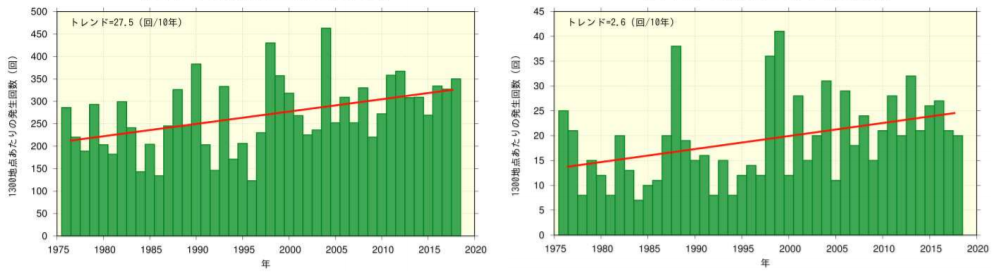
\includegraphics[width=1.0\linewidth,clip]{fig/intro/kisyotyo-repo-chart50-80.png}
		\subcaption{50mm(左)、80mm(右)}
		\label{a}
		\end{center}
		\end{minipage}\\
		
		\begin{minipage}[t]{1.0\hsize}	
		\begin{center}
		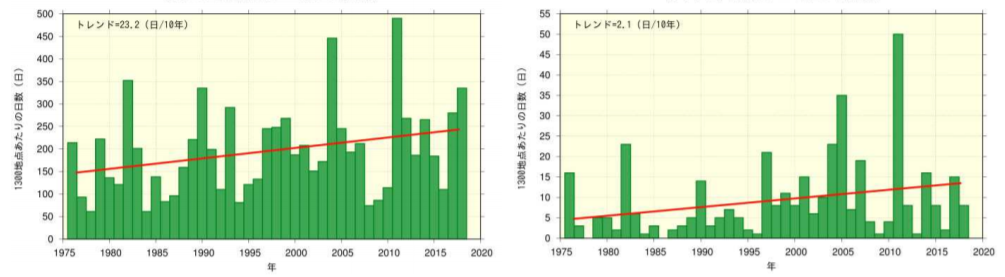
\includegraphics[width=1.0\linewidth,clip]{fig/intro/kisyotyo-repo-chart200-400.png}
		\subcaption{200mm(左)、400mm(右)}
		\label{b}
		\end{center}
		\end{minipage}
	\end{tabular}
	\caption{1976-2018年期間の全国のアメダスの1時間降水量50mm、80mm (a)、200mm、400mm (b) 以上の年間発生回数の変化。棒グラフは全国のアメダスによる観測値を 1300 地点当たりに換算した値、直線は長期変化傾向を表す。}
\end{figure}

Fumikai \textit{et al}.[2006]は、国内51地点の104年間(1901~2004年)の日降水量の資料
から日降水量の降水階級、100mm以上の日数、年最大降水量、年間の上位100事例の
発生頻度等の様々な大雨の尺度を用いて経年変化を調べた。いずれの尺度においても大雨の数は
増加傾向にあることがわかる。

\begin{figure}[H]
\begin{center}
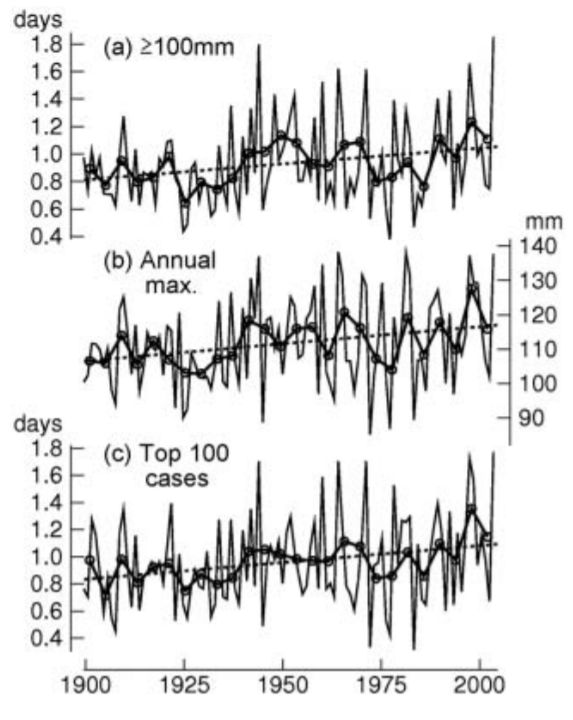
\includegraphics[width=0.8\linewidth]{fig/intro/fumikai-et-al-chart1.png}
\caption{1901-2004年期間の極端豪雨の経年変化:100mm以上の日数、年最大降水量、累年の上位100事例の発生頻度の時系列を示す。横軸は年。}
\end{center}
\end{figure}